\section{Ход работы}
\addcontentsline{toc}{section}{Ход работы}	% Добавляем его в оглавление

\begin{enumerate}
\item
Сборка измерительных приборов по схеме на рис ~\ref{sch2} без нулевого провода:

\begin{figure}[h]
\begin{center}
  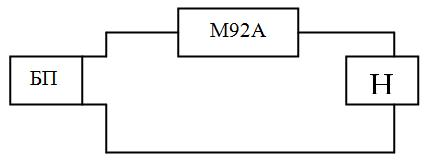
\includegraphics[width=0.3\linewidth]{scheme2}
  \caption{\label{sch2}}
\end{center}
\end{figure}

\item
Установим в фазах приёмника нагрузки в соответствии с данными таблицы. С помощью вольтметра измерим фазные и линейные напряжения, а также напряжение смещения нейтрали. Измерим фазные токи и мощности $ P_{1} $ и $ P_{2} $.

\item
  Изменяя количество нагрузочных элементов в регулируемой фазе, повторим измерения по пункту 2 для различных режимов. Результаты измерений занесем в таблицу:

\begin{table} [htbp]
  \centering
  \begin{tabular}{| p{0.6cm} | p{3cm} | p{0.6cm} | p{0.6cm} | p{0.6cm} | p{0.5cm} | p{0.5cm} | p{0.5cm} | p{0.6cm} | p{0.6cm} | p{0.6cm} | p{0.6cm} | p{0.5cm} | p{0.5cm} | p{0.5cm}l |}
  \hline

  \centering №, пп &\centering Режим работы &\centering $ U_{AB} $, B &\centering $ U_{BC} $, B &\centering $ U_{CA} $, B &\centering  $ U_{A} $, B &\centering $ U_{B} $, B &\centering  $ U_{C} $, B &\centering $ I_{A} $, мA &\centering $ I_{B} $, мA &\centering $ I_{C} $, мA &\centering $ U_{Nn} $, B &\centering $ P_{1} $, Вт &\centering $ P_{2} $, Вт &\centering  $ P $, Вт & \\

  \hline

  \centering 1 &\centering Симметричный &\centering 32 &\centering 28,5 &\centering 30,3 &\centering 18,1 &\centering 17,2 &\centering 17,3 &\centering 255 &\centering 240 &\centering 230 &\centering 0,9 &\centering 7,5 &\centering 7,5 &\centering 22,5 & \\

  \hline

  \centering 2 &\centering Обрыв фазы &\centering 12,7 &\centering 28,5 &\centering 15,7 &\centering 28,7 &\centering 13,2 &\centering 15,3 &\centering 0 &\centering 180 &\centering 210 &\centering 9,4 &\centering 8,5 &\centering -- &\centering 8,5 & \\

  \hline

  \centering 3 &\centering Короткое замыкание &\centering 30,6 &\centering 28,4 &\centering 29,4 &\centering 0,03 &\centering 30,7 &\centering 29,2 &\centering 740 &\centering 420 &\centering 410 &\centering 17,5 &\centering 35 &\centering 7,5 &\centering 42,5 &\\

  \hline

  \centering 4 &\centering Сопротивление увеличено &\centering 32,2 &\centering 28,3 &\centering 30,4 &\centering 22,5 &\centering 15,1 &\centering 15,9 &\centering 170 &\centering 200 &\centering 200 &\centering 3,6 &\centering 7,5 &\centering 7,5 &\centering 16 & \\

  \hline

  \centering 5 &\centering Сопротивление уменьшено &\centering 31,7 &\centering 30,3 &\centering 28,6 &\centering 14,2 &\centering 19,8 &\centering 19,4 &\centering 350 &\centering 270 &\centering 250 &\centering 4,2 &\centering 7,5 &\centering 17,5 &\centering 25 & \\

  \hline

  \centering 6 &\centering Домашнее задание &\centering &\centering &\centering &\centering &\centering &\centering &\centering &\centering &\centering &\centering &\centering &\centering &\centering & \\

  \hline

  \end{tabular}
  \caption{Результаты измерений для трехфазной цепи без нулевого провода}
\end{table}

\item
По данным таблицы построим векторные диаграммы токов и напряжений:

\vspace{70mm}

\item
Повторим измерения для трехфазной цепи с нулевым проводом. Результаты измерений занесем в таблицу:

\begin{table} [htbp]
  \centering
  \begin{tabular}{| p{0.8cm} | p{3cm} | p{0.8cm} | p{0.8cm} | p{0.8cm} | p{0.8cm} | p{0.8cm} | p{0.8cm} | p{0.8cm} | p{0.8cm} | p{0.8cm} | p{0.8cm}l |}
  \hline

  \centering №, пп &\centering Режим работы &\centering $ U_{AB} $, B &\centering $ U_{BC} $, B &\centering $ U_{CA} $, B &\centering  $ U_{A} $, B &\centering $ U_{B} $, B &\centering  $ U_{C} $, B &\centering $ I_{A} $, мA &\centering $ I_{B} $, мA &\centering $ I_{C} $, мA &\centering $ I_{N} $, мA & \\

  \hline

  \centering 1 &\centering Симметричный &\centering 32,2 &\centering 28,7 &\centering 30,6 &\centering 18,6 &\centering 17,5 &\centering 16,7 &\centering 260 &\centering 250 &\centering 240 &\centering 0 & \\

  \hline

  \centering 2 &\centering Обрыв фазы &\centering 32,3 &\centering 28,6 &\centering 31,1 &\centering 19,6 &\centering 17,2 &\centering 16,6 &\centering 0 &\centering 250 &\centering 230 &\centering 260 & \\

  \hline

  \centering 3 &\centering Сопротивление увеличено &\centering 32,5 &\centering 28,8 &\centering 30,9 &\centering 19,1 &\centering 17,4 &\centering 16,7 &\centering 140 &\centering 250 &\centering 210 &\centering 0,15 & \\

  \hline

  \centering 4 &\centering Сопротивление уменьшено &\centering 31,9 &\centering 28,9 &\centering 30,4 &\centering 18,0 &\centering 18,0 &\centering 16,7 &\centering 440 &\centering 250 &\centering 210 &\centering 0,18 & \\

\hline

  \centering 5 &\centering Домашнее задание &\centering &\centering &\centering &\centering &\centering &\centering &\centering &\centering &\centering &\centering & \\

  \hline
  \end{tabular}
  \caption{Результаты измерений для трехфазной цепи c нулевым проводом}
\end{table}

\item
По данным таблицы построим векторные диаграммы токов и напряжений:

\vspace{70mm}

\end{enumerate}
\clearpage
